\documentclass[12pt, a4paper, twoside]{article}

\usepackage[utf8]{inputenc}
\usepackage{tikz}

\title{Hausaufgabe 3}
\author{Aaron Sastry}

\begin{document}
	
	\maketitle
	
	\textbf{Aufgabe 3.1 Radix-Sort}
	\begin{description}
	
	\item [a)] \hfill \\
	Sortieren Sie die Folge a = (271, 842, 172, 828, 904, 023, 991, 800, 601, 889) mit LSD–
	RadixSort
	
	\emph{1st 10 buckets}
	\begin{tabular}{| c| c| c| c| c| c| c| c| c| c|}
		
		\hline
		B0 & B1 & B2 & B3 & B4 & B5 & B6 & B7 & B8 & B9 \\
		\hline\hline
		
		800 & 271 & 842 & 023 & 904 & & & & 828 & 889  \\
		    & 991 & 172 & & & & & & &  \\
		    & 601 & & & & & & & & \\ 
		\hline
	\end{tabular}

	output 1: (800, 271, 991, 601, 842, 172, 023, 904, 828, 889)
	\newline
	
	\emph{2nd 10 buckets}
	\begin{tabular}{| c| c| c| c| c| c| c| c| c| c|}
		
		\hline
		B0 & B1 & B2 & B3 & B4 & B5 & B6 & B7 & B8 & B9 \\
		\hline\hline
		
		800 & & 023 & & 842 & & & 271 & 889 & 991 \\
		601 & & 828 & &     & & & 172 & & \\
		904 & & & &     & & &     & & \\
		\hline
	\end{tabular}
	
	output 2: (800, 601, 904, 023, 828, 842, 271, 172, 889, 991)
	\newline
	
	\emph{3rd 10 buckets}
	\begin{tabular}{| c| c| c| c| c| c| c| c| c| c|}
		
		\hline
		B0 & B1 & B2 & B3 & B4 & B5 & B6 & B7 & B8 & B9 \\
		\hline\hline
		
		023 & 172 & 271 & & & & 601 & & 800 & 904 \\
		    &     &     & & & &     & & 828 & 991 \\
		    &     &     & & & &     & & 842 &     \\
		    &     &     & & & &     & & 889 &     \\
		
		\hline
	\end{tabular}
	
	output 3: (023, 172, 271, 601, 800, 828, 842, 889, 904, 991)
	\newline
	\emph{Nach 3 Iterationen ist die List final sortiert mit der Reihenfolge:}
	\newline
	\textbf{\emph{023, 172, 271, 601, 800, 828, 842, 889, 904, 991}}
	\newline
	
	\pagebreak
	
	\item[b)] \hfill \\
	Sortieren Sie die Folge b = (0.271, 0.842, 0.172, 0.828, 0.904) mit MSD–RadixSort.
	\\ \\
	
	\emph{1st set of buckets}\\
	\begin{tabular}{| c| c| c| c| c| c| c| c| c| c|}
		
		\hline
		B0 & B1 & B2 & B3 & B4 & B5 & B6 & B7 & B8 & B9 \\
		\hline\hline
		
		& 0.172 & 0.271 & & & & & & 0.842 & 0.904 \\
		&       &       & & & & & & 0.828 &  \\
		
		\hline
	\end{tabular}

	output: 1 = ([0.172], [0.271], [0.842, 0.828], [0.904]) \\
	
	Jetzt werden nur noch die Buckets sortiert die mehr als 1 Element haben.
	
	\emph{2nd set of buckets, }
	\emph{(the 0.8 bucket)}\\
	\begin{tabular}{| c| c| c| c| c| c| c| c| c| c|}
		
		\hline
		B0 & B1 & B2 & B3 & B4 & B5 & B6 & B7 & B8 & B9 \\
		\hline\hline
		
		& & 0.828 & & 0.842 & & & & & \\
		
		\hline
	\end{tabular}
	
	output: ([0.172], [0.271], [[0.828], [0.842]], [0.904]) \\
	
	Zu guter Letzt werden jetzt noch die Buckets wieder zu einer fertigen Liste zusammen gesetzt:
	
	\textbf{$\Longrightarrow$ \emph{0.172, 0.271, 0.828, 0.842, 0.904}}
	
	
	\item[c)] \hfill \\
	Angenommen, Sie wollen m-stellige Binärzahlen mit MSD-RadixSort sortieren, wobei
	die Behälter rekursiv wieder mit MSD-RadixSort sortiert werden sollen. Was ist die
	Laufzeit dieses Sortieralgorithmus für n Binärzahlen, abhängig von n und m? Begründen
	Sie Ihre Behauptung kurz.
	\newline
	
	
	\textbf{Antwort:}
	\newline
	Aus jeder liste entstehen immmer 2 buckets auf denen wieder sortiert werden muss.
	Somit sind in der iteration i etwa : \(2^i\)  befüllte Buckets.
	Da alle Buckets vereinigt wieder genau n Elemente haben ist jede Iteration in
	\begin{center}
		\(T = n\)
	\end{center} 
	Nun gibt es natürlich etwa \(2^m\) Buckets und exakt \emph{m} operationen da dies die Anzahl der stellen sind in die wir einteilen.
	Somit erfolgt die Einteilung in die gesammten Buckets in
	\begin{center}
		 \(T = m*n\)
	\end{center}
	Zu guter Letzt fehlt noch die vereinigung der Buckets wieder in eine vollsändige List, was wieder genau \(T = n\)
	braucht. 
	Somit ist die finale Laufzeit bei:
	\begin{center}
		\item\(T = (m+1)*n \) \(\Longleftrightarrow T = m*n + n\)
		\item \emph{\( \Longrightarrow \mathcal{O}(m*n) \)}\\
	\end{center}
	\end{description}



	\textbf{Aufgabe 3.2 Heaps}
	\begin{description}
		\item[a)] Fügen Sie die Werte 10, 4, 3, 15, 21, 2, 8, 11 und 1 in einen anfangs leeren Heap ein.
		Stellen Sie nach jeder Einfüge-Operation den Heap als Baum dar und geben Sie das Array an, welches dem fertigen Heap entspricht.
		\\
		
		\emph{insert: 10}\\
		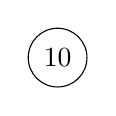
\begin{tikzpicture}
			\node[circle,draw](z){$10$};
		\end{tikzpicture}
		\\
		\emph{insert: 4}\\
		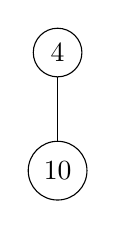
\begin{tikzpicture}
			\node[circle,draw](z){$4$}
			child{
				node[circle,draw]{10}};
		\end{tikzpicture}
		\\
		\emph{insert: 3}\\
		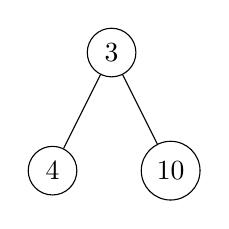
\begin{tikzpicture}
			\node[circle,draw](z){$3$}
			child{ node[circle,draw]{4}}
			child{node[circle,draw]{10}};
		\end{tikzpicture}
		\\
		\newpage
		\emph{insert: 15}\\
		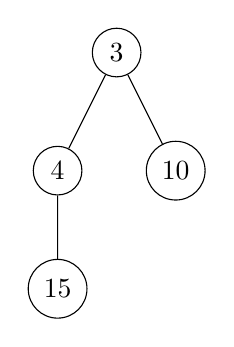
\begin{tikzpicture}
			\node[circle,draw](z){$3$}
			child{
				node[circle,draw]{4}  child{node[circle,draw]{15}}}
			child{node[circle,draw]{10}};
		\end{tikzpicture}
		\\
		\emph{insert: 21}\\
		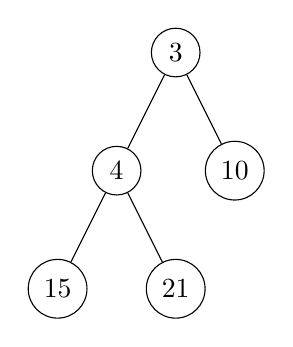
\begin{tikzpicture}
			\node[circle,draw](z){$3$}
			child{
				node[circle,draw]{4}  child{node[circle,draw]{15}} child{node[circle,draw]{21}}}
			child{node[circle,draw]{10}};
		\end{tikzpicture}
		\\
		\emph{insert: 2}\\
		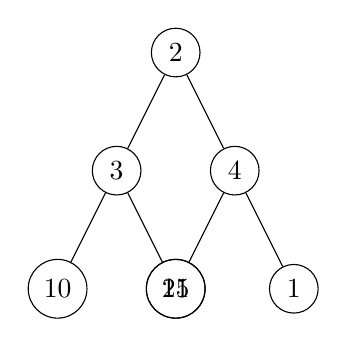
\begin{tikzpicture}
			\node[circle,draw](z){$2$}
			child{
				node[circle,draw]{3}  
					child{node[circle,draw]{10}} 
					child{node[circle,draw]{15}}}
			child{
				node[circle,draw]{4} 
					child{node[circle,draw]{21}} 
					child{node[circle,draw]{1}}};
		\end{tikzpicture}
		
		\item[b)] Führen Sie auf dem soeben gebauten Heap zwei deleteMin-Operationen durch und
		geben Sie jeweils den resultierenden Heap in Baumdarstellung und als Array an.
		
		\item[c)] Beschreiben Sie einen Algorithmus, der k sortierte Listen mit Gesamtlänge n in
		O(n log k) Zeit zu einer sortierten Liste zusammenfügt. Benutzen Sie dabei einen Heap.
		Begründen Sie kurz, dass Ihr Algorithmus die Laufzeitschranke einhält.
		
		\item[d)] Gegeben sei die folgende alternative Prozedur zum Erstellen eines binären Heaps für
		ein unsortiertes Array A[1..n]:
		buildHeapInsert(A : Array):
		1 for i ← 1 to n do
		2 insert(A[i])
		Geben Sie ein Beispiel für eine Eingabe an, sodass buildHeapInsert eine schlechtere
		Laufzeit für das Aufbauen des Heaps hat als O(n). Was ist die worst–case Laufzeit von
		buildHeapInsert? Begründen Sie!
		
	\end{description}
	
	
	
\end{document}